% Created 2016-09-23 Sex 14:32
\documentclass[11pt]{article}
\usepackage[utf8]{inputenc}
\usepackage[T1]{fontenc}
\usepackage{fixltx2e}
\usepackage{graphicx}
\usepackage{longtable}
\usepackage{float}
\usepackage{wrapfig}
\usepackage{rotating}
\usepackage[normalem]{ulem}
\usepackage{amsmath}
\usepackage{textcomp}
\usepackage{marvosym}
\usepackage{wasysym}
\usepackage{amssymb}
\usepackage{hyperref}
\tolerance=1000
\author{Cecília Carneiro e Silva}
\date{}
\title{TCC}
\hypersetup{
  pdfkeywords={},
  pdfsubject={},
  pdfcreator={Emacs 24.5.1 (Org mode 8.2.10)}}
\begin{document}

\maketitle
\tableofcontents


\section{TEMA}
\label{sec-1}

Maquina virtual em sitemas embacados

\section{TITULO}
\label{sec-2}

Sistema de virtualização para sistemas embarcados, utilizando a linguagem de programação Scheme.

\section{OBJETIVO GERAL}
\label{sec-3}


\section{SCHEME}
\label{sec-4}

Scheme

Scheme is a statically scoped and properly tail-recursive dialect of the Lisp programming language invented by Guy Lewis Steele Jr. and Gerald Jay Sussman. It was designed to have an exceptionally clear and simple semantics and few different ways to form expressions. A wide variety of programming paradigms, including imperative, functional, and message passing styles, find convenient expression in Scheme.

Scheme was one of the first programming languages to incorporate first class procedures as in the lambda calculus, thereby proving the usefulness of static scope rules and block structure in a dynamically typed language. Scheme was the first major dialect of Lisp to distinguish procedures from lambda expressions and symbols, to use a single lexical environment for all variables, and to evaluate the operator position of a procedure call in the same way as an operand position. By relying entirely on procedure calls to express iteration, Scheme emphasized the fact that tail-recursive procedure calls are essentially goto's that pass arguments. Scheme was the first widely used programming language to embrace first class escape procedures, from which all previously known sequential control structures can be synthesized. More recently, building upon the design of generic arithmetic in Common Lisp, Scheme introduced the concept of exact and inexact numbers. Scheme is also the first programming language to support hygienic macros, which permit the syntax of a block-structured language to be extended reliably.


\section{{\bfseries\sffamily DONE} PICOBIT - pdf}
\label{sec-5}

Terminar de ler o artigo oficial do picobit.

\subsection{{\bfseries\sffamily DONE} Foto folha}
\label{sec-5-1}

\begin{itemize}
\item GOOGLE-PHOTOS

Tirar foto da folha.

\item SIXPIC C compiler é somente para PIC18.
\item Nesse caso vamos usar o cross-compiler: arm-none-eabi-gcc.
\end{itemize}

\subsection{{\bfseries\sffamily TODO} Comentarios}
\label{sec-5-2}

\begin{itemize}
\item Por causa do ambiente com tamanho de codigo limitado, todo projeto foi voltado a gerar bytecode compact code.
\item O bytecode resultante da scheme compiler é menor q o machine code, ou seja, o tamanho da entrada da VM é menor q a saída.
\item Como o projeto tem total controle, virtual machine e C compiler, podemos adaptar um ao outro.
\item A maquina virtual é escrita em C, tornando fácil a portabilidade entre hardwares, esse trabalho: STM32F1 e STM32F4.
\end{itemize}

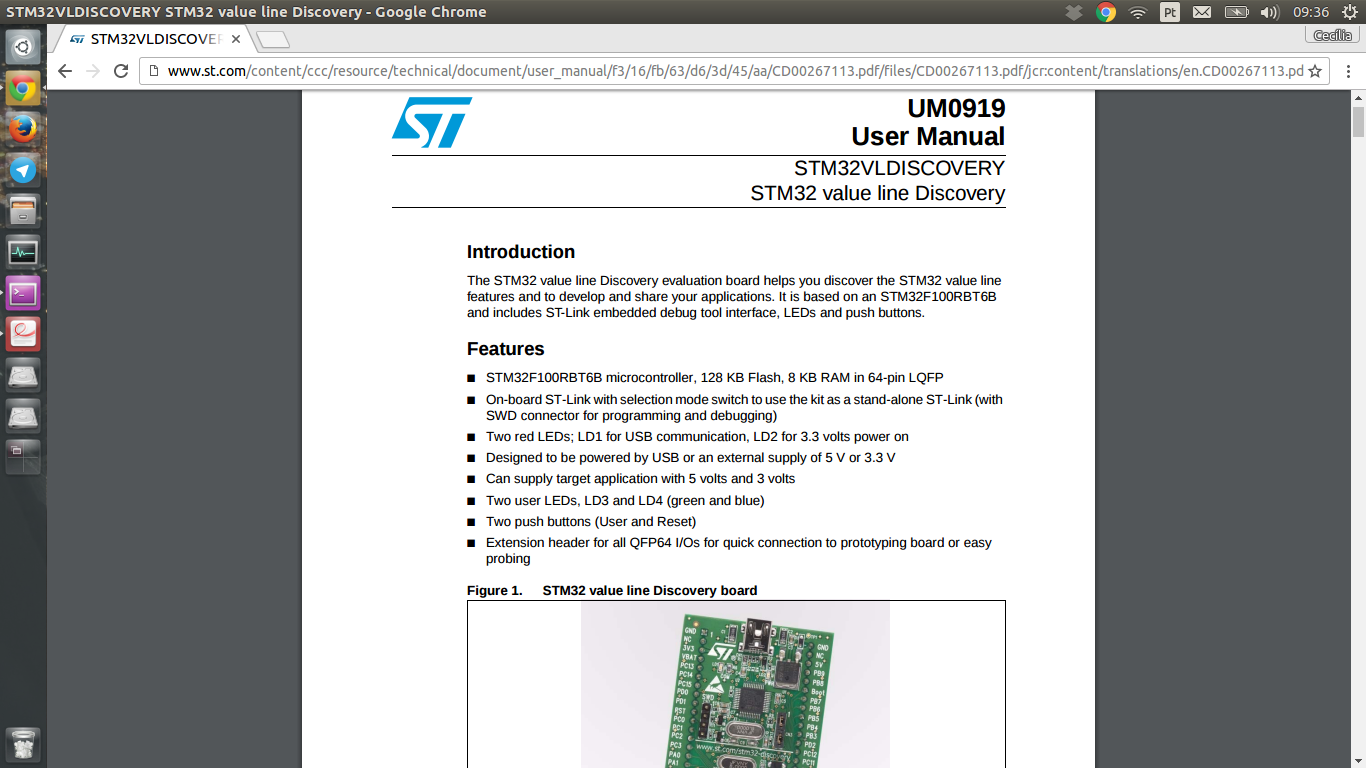
\includegraphics[width=.9\linewidth]{stm32f1.png}


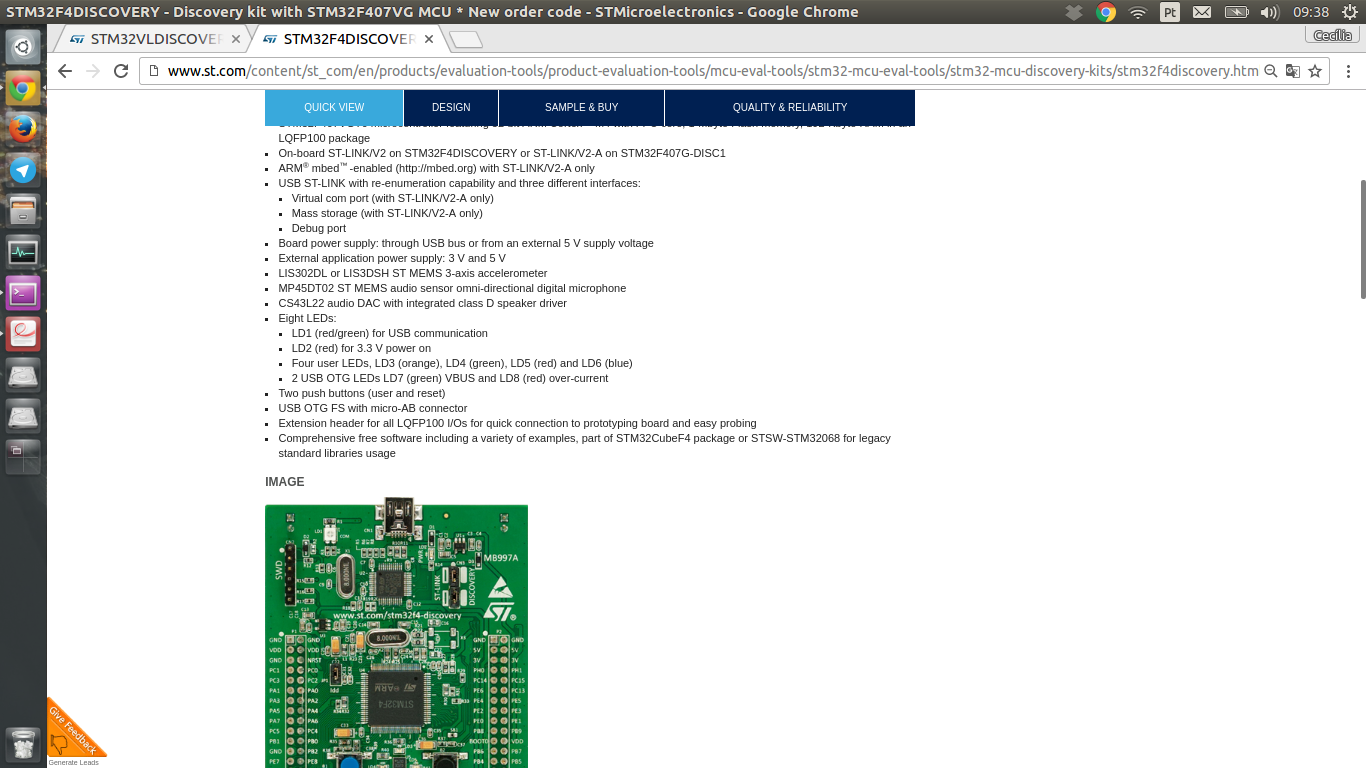
\includegraphics[width=.9\linewidth]{stm32f4.png}

\begin{itemize}
\item Implementação do R5RS, tem: macros, closures, listas, gerenciamento de memória, predicados de alta ordem, inteiros de precisão, strings, etc.
\item Não foi implementado (visando ser mais compacto, são coisa não uteis em Embedded Systems-ES): ponto flutuante, file I/O, eval, rational, complex numbers, symbol->string, string->symbol.
\item Suporte à listas.
\item The term continuations can also be used to refer to first-class continuations, which are constructs that give a programming language the ability to save the execution state at any point and return to that point at a later point in the program, possibly multiple times.
\end{itemize}

\subsubsection{{\bfseries\sffamily DONE} PICOBIT-SCHEME compiler}
\label{sec-5-2-1}

Compilador Scheme especializado em gerar bytecode otimizado. Programa acoplado com a biblioteca, então o bytecode é gerado dos dois juntos resultando em um bytecode mais compacto quando comparado a versão separada.

Conjunto de instações compartilhadas pelo compiler e pela VM, criado e planejado para essa aplicação, todos optimizações voltadas a isso.

\begin{itemize}
\item Para diminuir as alocações em tempo de execução (alocações dinamicas), toda analise de mutabilidade é feita em tempo de compilação, variáveis que nao alteram o valor não são alocadas na memória.   --   startup.s
\item Enfim, compiler e linker são feitos na mesma etapa.
\item Branchs consecutivos são pulandos, importando apenas o final.
\end{itemize}

\subsubsection{{\bfseries\sffamily TODO} PICOBIT bytecode}
\label{sec-5-2-2}

\begin{itemize}
\item PICOBIT é uma maquina virtual de pilha (stack-based virtual machine).
\item Não entendi mto bem nao.
\end{itemize}

\subsubsection{{\bfseries\sffamily TODO} PICOBIT-virtual machine}
\label{sec-5-2-3}

É a parte do picobit voltada ao microcontrolador. É o interpletador do bytecode gerado pelo scheme compiler.

\begin{itemize}
\item Pensanda para ser o mais compacta possível.
\item Inclui coletor de lixo, número com precisão e suporte a estruturas de dados.
\item Stack based, cons of cells.
\end{itemize}

\begin{enumerate}
\item Mark-and-Sweep Garbage Collection
\label{sec-5-2-3-1}

When using mark-and-sweep, unreferenced objects are not reclaimed immediately. Instead, garbage is allowed to accumulate until all available memory has been exhausted. When that happens, the execution of the program is suspended temporarily while the mark-and-sweep algorithm collects all the garbage. Once all unreferenced objects have been reclaimed, the normal execution of the program can resume.

The mark-and-sweep algorithm is called a tracing garbage collector because is traces out the entire collection of objects that are directly or indirectly accessible by the program. The objects that a program can access directly are those objects which are referenced by local variables on the processor stack as well as by any static variables that refer to objects. In the context of garbage collection, these variables are called the roots . An object is indirectly accessible if it is referenced by a field in some other (directly or indirectly) accessible object. An accessible object is said to be live . Conversely, an object which is not live is garbage.

The mark-and-sweep algorithm consists of two phases: In the first phase, it finds and marks all accessible objects. The first phase is called the mark phase. In the second phase, the garbage collection algorithm scans through the heap and reclaims all the unmarked objects. The second phase is called the sweep phase.

\item Copying garbage collection
\label{sec-5-2-3-2}

Usa apenas metade da memoria, copia de uma parte para outra.
Mais complicado q o Mark-and-sweet collection.

\begin{itemize}
\item Normalmente os microcontroladores tem mais ROM quem RAM, então é interessante passar td que é possivel para a ROM, deixando na RAM somente os dados mutáveis.
\item Variaves com valor conhecido em compile-time são colocados na ROM, PICOBIT consegue manipular obbjetos tanto da ROM quanto da RAM.
\item full version = 13-bit encoding
\item ligth version = 8-bit-encoding
\item Unbounded precision integer type são providos, So unbounded in this context means bounded only by the availability of system resources; there is no hard-coded limit to the number of digits in the value that an unbounded-precision integer type an represent. Permite que o PICOBIT implemente protocolos de redes que necessitam, por exemplo, do MAC adress (48 bits) ou  SHA criptografia.
\end{itemize}
\end{enumerate}

\section{{\bfseries\sffamily TODO} R5RS}
\label{sec-6}

Descrição da linguagem de programação Scheme. Linguagem fracamente tipada, ou dinamicamente tipada, latent type.

Scheme was one of the first languages to support procedures as objects in their own right. Procedures can be created dynamically, stored in data structures, returned as results of procedures, and so on. Other languages with these properties include Common Lisp, Haskell, ML, Ruby, and Smalltalk.

Scheme por definição é uma linguage weak, não lazy.

Scheme programms manipulam objetos também conhecidos como valores. 

\section{{\bfseries\sffamily TODO} Compiler files study}
\label{sec-7}
Estudo e análise dos codigos do compilador PICOBIT, scheme to bytecode.

\subsection{{\bfseries\sffamily TODO} Objective}
\label{sec-7-1}
Primeiro objetivo é atualizar para a versão 6.6 do Racket. Atualmente está rodando na versão 6.2 do racket, com modificação no arquivo port.rkt, unstable.

\subsection{Utilities}
\label{sec-7-2}

\begin{itemize}
\item SRFI/4 = vetores numéricos homogênios
= Marc Feeley
= vetores numericos em que todos os elementos tem o mesmo tipo.
= vetores homogenios devem ser usado em comunicação com bibliotecas de baixo nível.
= 8 tipos de vetores homogênios inteiros, 2 tipos de ponto flutuante.

\item todas funções visiveis fora do arquivo.
\item parameterize = cria um novo thread com aquela variável.
\end{itemize}

\subsection{Env}
\label{sec-7-3}

\begin{itemize}
\item require: utilities.rkt
\item provide all.
\item Toda estruturação das variaveis e funcoes. Enfim estruturação do ambiente de compilação.
\end{itemize}

\subsection{Ast}
\label{sec-7-4}
\begin{itemize}
\item require utilities.rkt env.rkt
\item provide all.
\item objetos com multiplas relações, defs, refs, sets e prcs.
\end{itemize}

\subsubsection{{\bfseries\sffamily TODO} unstable/match}
\label{sec-7-4-1}

Tirar isso, tornar estavel, compartivel com a ultima versão do racket.

\begin{itemize}
\item entre outras coisas, verifica se a variavel é mutável ou nao.
\end{itemize}


\section{{\bfseries\sffamily TODO} ARM - livro}
\label{sec-8}

Joseph Yiu (Auth.)-The Definitive Guide to Arm® Cortex®-M3 and Cortex®-M4 Processors-Newnes (2014).pdf

\section{{\bfseries\sffamily TODO} tanenbaum - book}
\label{sec-9}

Operating systems.

\section{{\bfseries\sffamily TODO} Virtual machines}
\label{sec-10}

\section{{\bfseries\sffamily TODO} PICOBIT SCHEME COMPILER}
\label{sec-11}

\section{{\bfseries\sffamily TODO} PICOBIT VM}
\label{sec-12}

\section{{\bfseries\sffamily TODO} SIXPIC C COMPILER}
\label{sec-13}
% Emacs 24.5.1 (Org mode 8.2.10)
\end{document}
